\chapter[Sprint V]{Study and Implementation of Sprint V: Community Interaction \& Profile Management}

\minitoc

\section{Introduction}

Sprint V marks a significant milestone in our platform development, focusing on building a vibrant community ecosystem and enhancing user profile management capabilities. This sprint introduces comprehensive community interaction features that enable users to engage with shared projects through comments, likes, and collaborative copying mechanisms. Additionally, we implement robust profile management functionality that allows users to maintain their digital presence and showcase their work effectively.

The community interaction features transform our platform from a simple diagramming tool into a collaborative workspace where users can discover, learn from, and build upon each other's work. The profile management system provides users with the tools to curate their professional presence and manage their project portfolios efficiently.

\section{Sprint Planning}

\subsection{Objectives of Sprint V}

The primary objectives of Sprint V are to establish a comprehensive community interaction system and implement essential profile management features. These objectives include:

\begin{itemize}
\item Develop community exploration capabilities for both authenticated users and visitors
\item Implement project interaction features including commenting, liking, and sharing
\item Create comment management system with full CRUD operations
\item Enable project copying functionality for collaborative learning
\item Build comprehensive profile editing and management system
\item Implement public project viewing on user profiles
\end{itemize}

\subsection{Backlog of Sprint V}

\begin{table}[H]
\centering
\caption{Sprint V Product Backlog}
\begin{tabular}{|p{1cm}|p{8cm}|p{1.5cm}|p{1cm}|}
\hline
\textbf{ID} & \textbf{User Story} & \textbf{Feature} & \textbf{Size} \\
\hline
6.1 & As a user, I want to explore the community so that I can discover interesting projects. & Community Interaction & S \\
\hline
6.2 & As a visitor, I want to explore the community so that I can see what the platform offers. & Community Interaction & S \\
\hline
6.3 & As a user, I want to comment on projects so that I can provide feedback to other users. & Community Interaction & C \\
\hline
6.4 & As a user, I want to like/unlike projects so that I can show appreciation for good work. & Community Interaction & C \\
\hline
6.5 & As a user, I want to share projects so that I can promote interesting content. & Community Interaction & C \\
\hline
6.6 & As a user, I want to update my comments so that I can correct or improve my feedback. & Community Interaction & C \\
\hline
6.7 & As a user, I want to delete my comments so that I can remove inappropriate or outdated feedback. & Community Interaction & C \\
\hline
6.8 & As a user, I want to like/unlike comments so that I can engage in community discussions. & Community Interaction & C \\
\hline
6.9 & As a user, I want to copy community projects to my workspace so that I can learn from and build upon others' work. & Community Interaction & S \\
\hline
7.1 & As a user, I want to edit my profile so that I can keep my information current. & Profile Management & S \\
\hline
7.2 & As a user, I want to view public projects on profiles so that I can see others' work. & Profile Management & S \\
\hline
\end{tabular}
\end{table}

\section{Analyse}

\subsection{Use case diagram for sprint V}

\begin{figure}[H]
\centering
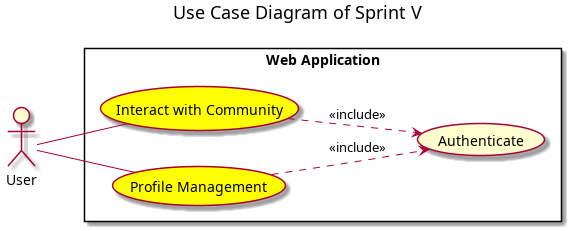
\includegraphics[width=0.9\textwidth]{conception/SprintV/use_case_diagrams/use_case_diagram_of_SprintV.png}
\caption{Use Case Diagram for Sprint V}
\label{fig:use_case_sprint_v}
\end{figure}

The overall use case diagram for Sprint V illustrates the complete ecosystem of community interaction and profile management features, showing the relationships between different actors and their associated use cases.

\subsection{Refined use case "Community Interaction"}

\begin{figure}[H]
\centering
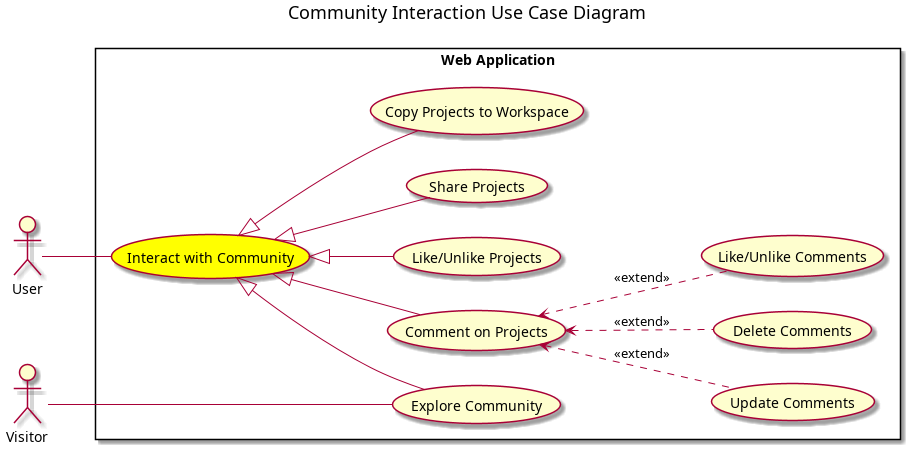
\includegraphics[width=0.9\textwidth]{conception/SprintV/use_case_diagrams/refined_use_case_feature_community_interaction.png}
\caption{Refined Use Case Diagram for Community Interaction Feature}
\label{fig:community_interaction_use_case}
\end{figure}

\subsubsection{Use case}

The community interaction feature encompasses multiple interconnected use cases:

\begin{itemize}
\item Explore Community
\item Comment on Projects
\item Like/Unlike Projects
\item Update Comments
\item Delete Comments
\item Like/Unlike Comments
\item Copy Projects to Workspace
\end{itemize}

\subsubsection{Textual description of use case "Explore community"}

\begin{table}[H]
\centering
\caption{Use Case: Explore Community}
\begin{tabular}{|p{3cm}|p{10cm}|}
\hline
\textbf{Use Case Name} & Explore Community \\
\hline
\textbf{Actor} & User, Visitor \\
\hline
\textbf{Description} & Users and visitors can browse through community projects to discover interesting content and see what the platform offers \\
\hline
\textbf{Preconditions} & Platform is accessible, community section is available \\
\hline
\textbf{Main Flow} & 
1. Actor accesses community section \\
& 2. System displays list of public projects \\
& 3. Actor can filter and search projects \\
& 4. Actor can view project details \\
& 5. System shows project metadata and interactions \\
\hline
\textbf{Alternative Flow} & If no projects available, system shows empty state message \\
\hline
\textbf{Postconditions} & Actor has viewed community projects \\
\hline
\textbf{Exceptions} & Network connectivity issues, server errors \\
\hline
\end{tabular}
\end{table}

\subsubsection{Textual description of use case "Comment on projects"}

\begin{table}[H]
\centering
\caption{Use Case: Comment on Projects}
\begin{tabular}{|p{3cm}|p{10cm}|}
\hline
\textbf{Use Case Name} & Comment on Projects \\
\hline
\textbf{Actor} & Authenticated User \\
\hline
\textbf{Description} & Users can add comments to projects to provide feedback and engage with the community \\
\hline
\textbf{Preconditions} & User is authenticated, project exists and is accessible \\
\hline
\textbf{Main Flow} & 
1. User navigates to project page \\
& 2. User clicks on comment section \\
& 3. User enters comment text \\
& 4. User submits comment \\
& 5. System validates and saves comment \\
& 6. System displays updated comment list \\
\hline
\textbf{Alternative Flow} & Comment validation fails, user must correct input \\
\hline
\textbf{Postconditions} & Comment is added to project \\
\hline
\textbf{Exceptions} & Invalid comment content, server errors, unauthorized access \\
\hline
\end{tabular}
\end{table}

\subsubsection{Textual description of use case "Like/Unlike projects"}

\begin{table}[H]
\centering
\caption{Use Case: Like/Unlike Projects}
\begin{tabular}{|p{3cm}|p{10cm}|}
\hline
\textbf{Use Case Name} & Like/Unlike Projects \\
\hline
\textbf{Actor} & Authenticated User \\
\hline
\textbf{Description} & Users can express appreciation for projects by liking or unliking them \\
\hline
\textbf{Preconditions} & User is authenticated, project exists and is accessible \\
\hline
\textbf{Main Flow} & 
1. User views project \\
& 2. User clicks like/unlike button \\
& 3. System toggles like status \\
& 4. System updates like count \\
& 5. System reflects change in UI \\
\hline
\textbf{Alternative Flow} & System handles rapid successive clicks appropriately \\
\hline
\textbf{Postconditions} & Project like status is updated \\
\hline
\textbf{Exceptions} & Server errors, unauthorized access \\
\hline
\end{tabular}
\end{table}

\subsubsection{Textual description of use case "Update comments"}

\begin{table}[H]
\centering
\caption{Use Case: Update Comments}
\begin{tabular}{|p{3cm}|p{10cm}|}
\hline
\textbf{Use Case Name} & Update Comments \\
\hline
\textbf{Actor} & Authenticated User \\
\hline
\textbf{Description} & Users can modify their existing comments to correct or improve their feedback \\
\hline
\textbf{Preconditions} & User is authenticated, user owns the comment, comment exists \\
\hline
\textbf{Main Flow} & 
1. User locates their comment \\
& 2. User clicks edit button \\
& 3. System displays editable comment form \\
& 4. User modifies comment text \\
& 5. User saves changes \\
& 6. System validates and updates comment \\
& 7. System displays updated comment \\
\hline
\textbf{Alternative Flow} & User cancels edit operation, comment remains unchanged \\
\hline
\textbf{Postconditions} & Comment is updated with new content \\
\hline
\textbf{Exceptions} & Validation errors, unauthorized edit attempt, server errors \\
\hline
\end{tabular}
\end{table}

\subsubsection{Textual description of use case "Delete comments"}

\begin{table}[H]
\centering
\caption{Use Case: Delete Comments}
\begin{tabular}{|p{3cm}|p{10cm}|}
\hline
\textbf{Use Case Name} & Delete Comments \\
\hline
\textbf{Actor} & Authenticated User \\
\hline
\textbf{Description} & Users can remove their comments to eliminate inappropriate or outdated feedback \\
\hline
\textbf{Preconditions} & User is authenticated, user owns the comment, comment exists \\
\hline
\textbf{Main Flow} & 
1. User locates their comment \\
& 2. User clicks delete button \\
& 3. System shows confirmation dialog \\
& 4. User confirms deletion \\
& 5. System removes comment \\
& 6. System updates comment list \\
\hline
\textbf{Alternative Flow} & User cancels deletion, comment is preserved \\
\hline
\textbf{Postconditions} & Comment is permanently removed \\
\hline
\textbf{Exceptions} & Unauthorized deletion attempt, server errors \\
\hline
\end{tabular}
\end{table}

\subsubsection{Textual description of use case "Like/Unlike comments"}

\begin{table}[H]
\centering
\caption{Use Case: Like/Unlike Comments}
\begin{tabular}{|p{3cm}|p{10cm}|}
\hline
\textbf{Use Case Name} & Like/Unlike Comments \\
\hline
\textbf{Actor} & Authenticated User \\
\hline
\textbf{Description} & Users can engage in community discussions by liking or unliking comments \\
\hline
\textbf{Preconditions} & User is authenticated, comment exists and is visible \\
\hline
\textbf{Main Flow} & 
1. User views comment \\
& 2. User clicks like/unlike button on comment \\
& 3. System toggles like status for comment \\
& 4. System updates comment like count \\
& 5. System reflects change in UI \\
\hline
\textbf{Alternative Flow} & System prevents liking own comments \\
\hline
\textbf{Postconditions} & Comment like status is updated \\
\hline
\textbf{Exceptions} & Server errors, unauthorized access \\
\hline
\end{tabular}
\end{table}

\subsubsection{Textual description of use case "Copy projects to workspace"}

\begin{table}[H]
\centering
\caption{Use Case: Copy Projects to Workspace}
\begin{tabular}{|p{3cm}|p{10cm}|}
\hline
\textbf{Use Case Name} & Copy Projects to Workspace \\
\hline
\textbf{Actor} & Authenticated User \\
\hline
\textbf{Description} & Users can copy community projects to their personal workspace for learning and building upon others' work \\
\hline
\textbf{Preconditions} & User is authenticated, project is public and copyable, user has workspace access \\
\hline
\textbf{Main Flow} & 
1. User views community project \\
& 2. User clicks copy to workspace button \\
& 3. System prompts for copy destination \\
& 4. User selects target workspace \\
& 5. System creates project copy \\
& 6. System notifies user of successful copy \\
& 7. System redirects to copied project \\
\hline
\textbf{Alternative Flow} & User cancels copy operation \\
\hline
\textbf{Postconditions} & Project copy exists in user's workspace \\
\hline
\textbf{Exceptions} & Insufficient permissions, storage limitations, server errors \\
\hline
\end{tabular}
\end{table}

\subsection{Refined use case "Profile Management"}

\begin{figure}[H]
\centering
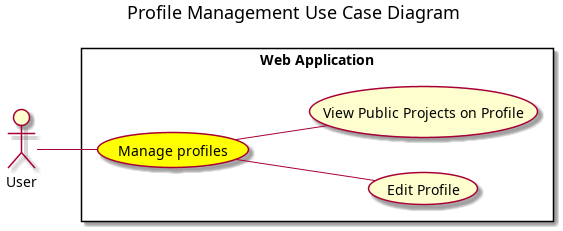
\includegraphics[width=0.9\textwidth]{conception/SprintV/use_case_diagrams/refined_use_case_feature_profiles .png}
\caption{Refined Use Case Diagram for Profile Management Feature}
\label{fig:profile_management_use_case}
\end{figure}

The profile management feature includes:

\begin{itemize}
\item Edit Profile
\item View Public Projects on Profile
\end{itemize}

\subsubsection{Textual description of use case "Edit profile"}

\begin{table}[H]
\centering
\caption{Use Case: Edit Profile}
\begin{tabular}{|p{3cm}|p{10cm}|}
\hline
\textbf{Use Case Name} & Edit Profile \\
\hline
\textbf{Actor} & Authenticated User \\
\hline
\textbf{Description} & Users can update their profile information to keep their account details current \\
\hline
\textbf{Preconditions} & User is authenticated and has access to profile settings \\
\hline
\textbf{Main Flow} & 
1. User navigates to profile settings \\
& 2. System displays current profile information \\
& 3. User modifies desired fields \\
& 4. User submits changes \\
& 5. System validates input \\
& 6. System updates profile data \\
& 7. System confirms successful update \\
\hline
\textbf{Alternative Flow} & Validation fails, user must correct invalid inputs \\
\hline
\textbf{Postconditions} & User profile is updated with new information \\
\hline
\textbf{Exceptions} & Validation errors, server errors, unauthorized access \\
\hline
\end{tabular}
\end{table}

\subsubsection{Textual description of use case "View Public Projects on Profile"}

\begin{table}[H]
\centering
\caption{Use Case: View Public Projects on Profile}
\begin{tabular}{|p{3cm}|p{10cm}|}
\hline
\textbf{Use Case Name} & View Public Projects on Profile \\
\hline
\textbf{Actor} & User, Visitor \\
\hline
\textbf{Description} & Users and visitors can view public projects displayed on user profiles to explore others' work \\
\hline
\textbf{Preconditions} & Profile exists and is accessible, user has public projects \\
\hline
\textbf{Main Flow} & 
1. Actor navigates to user profile \\
& 2. System displays profile information \\
& 3. System shows list of public projects \\
& 4. Actor can browse project thumbnails \\
& 5. Actor can click to view project details \\
\hline
\textbf{Alternative Flow} & If no public projects, system shows appropriate message \\
\hline
\textbf{Postconditions} & Actor has viewed user's public projects \\
\hline
\textbf{Exceptions} & Profile not found, server errors \\
\hline
\end{tabular}
\end{table}

\section{Conception}

The conception phase for Sprint V involves detailed sequence diagrams that illustrate the interaction flows for each implemented feature. These diagrams demonstrate how different system components collaborate to deliver the community interaction and profile management functionality.

\subsection{Community Interaction Sequence Diagrams}

\begin{figure}[H]
\centering
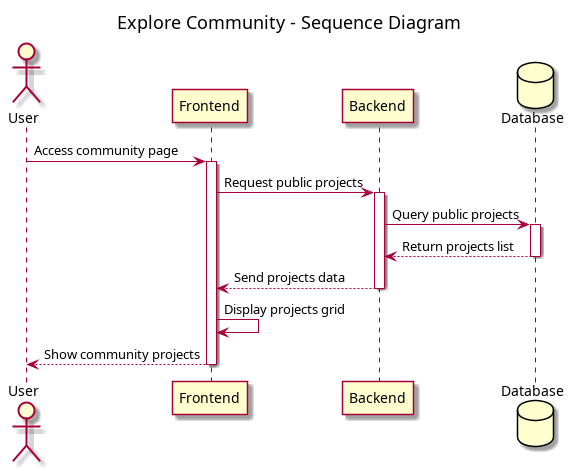
\includegraphics[width=0.9\textwidth]{conception/SprintV/sequence_diagrams/sequence_communityInteraction_6_1_ExploreCommunityAsUser.png}
\caption{Sequence Diagram: Explore Community as User}
\label{fig:seq_explore_community}
\end{figure}

\begin{figure}[H]
\centering
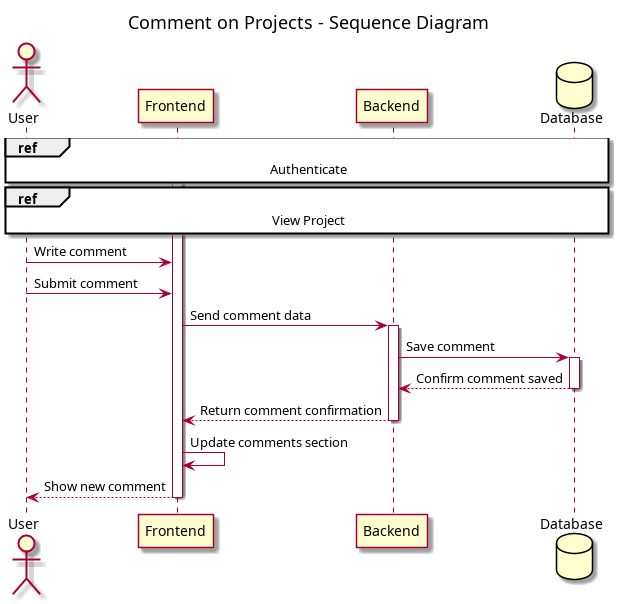
\includegraphics[width=0.9\textwidth]{conception/SprintV/sequence_diagrams/sequence_communityInteraction_6_3_CommentOnProjects.png}
\caption{Sequence Diagram: Comment on Projects}
\label{fig:seq_comment_projects}
\end{figure}

\begin{figure}[H]
\centering
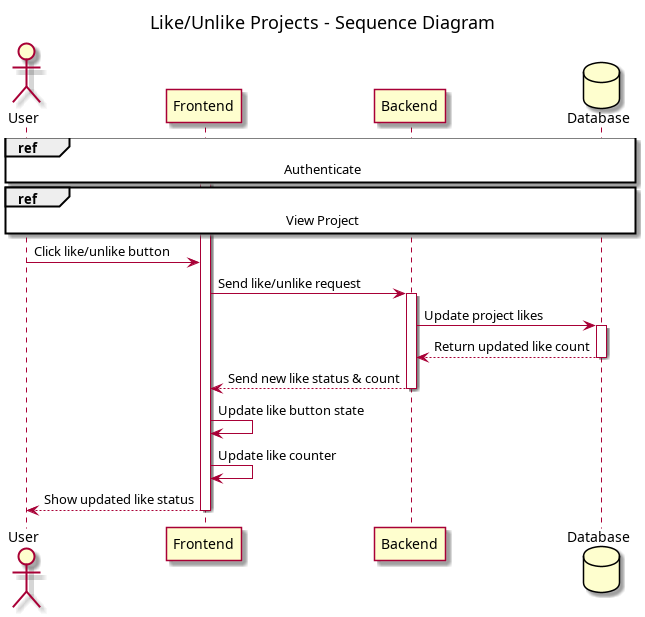
\includegraphics[width=0.9\textwidth]{conception/SprintV/sequence_diagrams/sequence_communityInteraction_6_4_LikeUnlikeProjects.png}
\caption{Sequence Diagram: Like/Unlike Projects}
\label{fig:seq_like_projects}
\end{figure}

\begin{figure}[H]
\centering
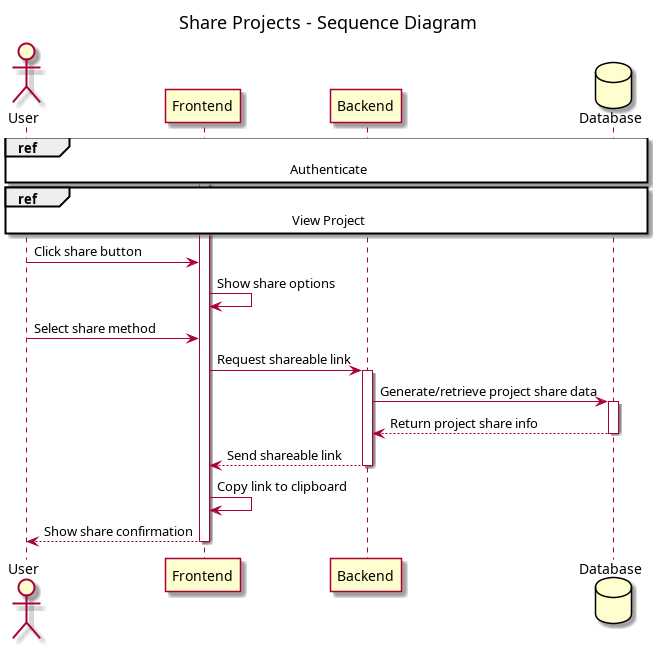
\includegraphics[width=0.9\textwidth]{conception/SprintV/sequence_diagrams/sequence_communityInteraction_6_5_ShareProjects.png}
\caption{Sequence Diagram: Share Projects}
\label{fig:seq_share_projects}
\end{figure}

\begin{figure}[H]
\centering
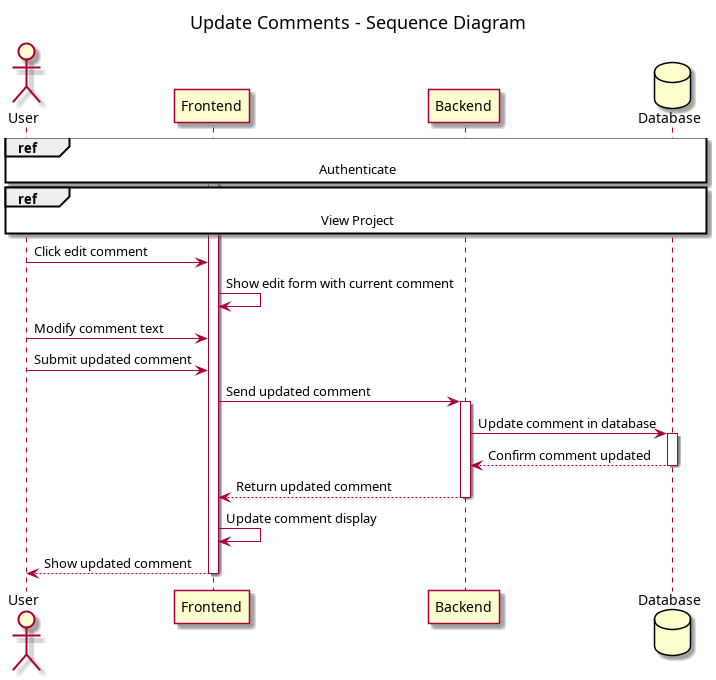
\includegraphics[width=0.9\textwidth]{conception/SprintV/sequence_diagrams/sequence_communityInteraction_6_6_UpdateComments.png}
\caption{Sequence Diagram: Update Comments}
\label{fig:seq_update_comments}
\end{figure}

\begin{figure}[H]
\centering
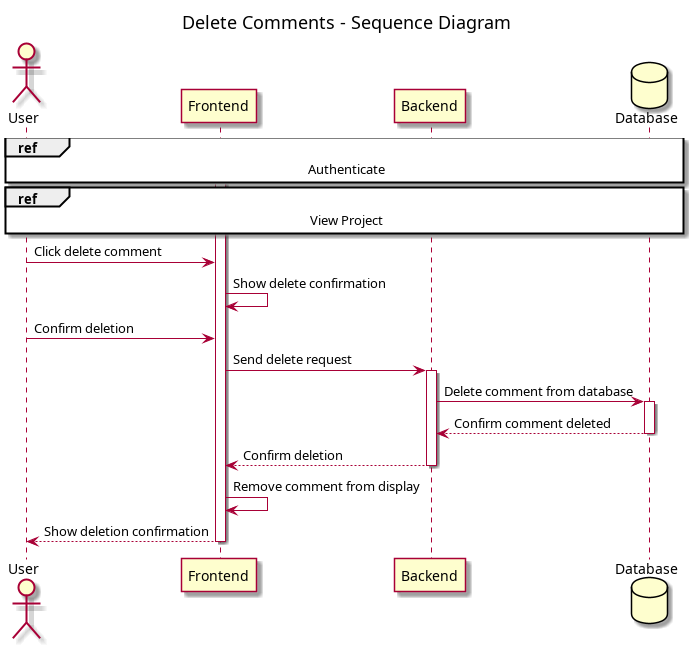
\includegraphics[width=0.9\textwidth]{conception/SprintV/sequence_diagrams/sequence_communityInteraction_6_7_DeleteComments.png}
\caption{Sequence Diagram: Delete Comments}
\label{fig:seq_delete_comments}
\end{figure}

\begin{figure}[H]
\centering
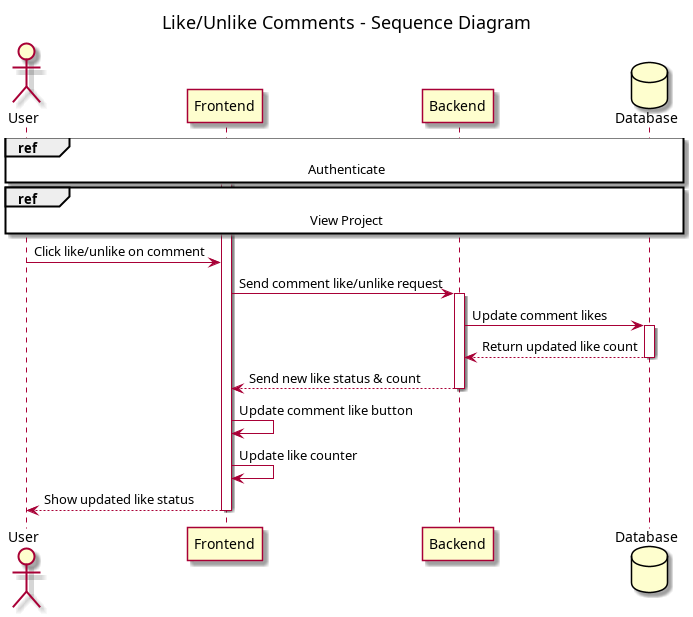
\includegraphics[width=0.9\textwidth]{conception/SprintV/sequence_diagrams/sequence_communityInteraction_6_8_LikeUnlikeComments.png}
\caption{Sequence Diagram: Like/Unlike Comments}
\label{fig:seq_like_comments}
\end{figure}

\begin{figure}[H]
\centering
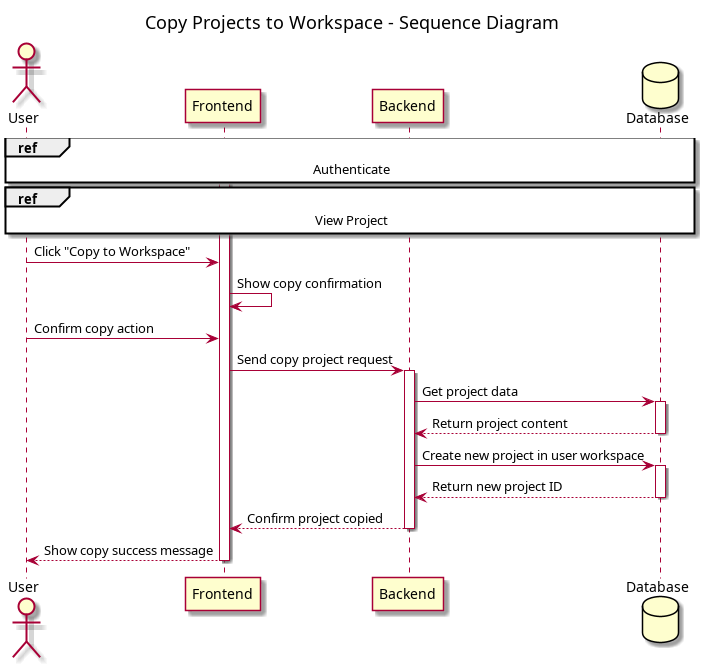
\includegraphics[width=0.9\textwidth]{conception/SprintV/sequence_diagrams/sequence_communityInteraction_6_9_CopyCommunityProjectsToWorkspace.png}
\caption{Sequence Diagram: Copy Community Projects to Workspace}
\label{fig:seq_copy_projects}
\end{figure}

\subsection{Profile Management Sequence Diagrams}

\begin{figure}[H]
\centering
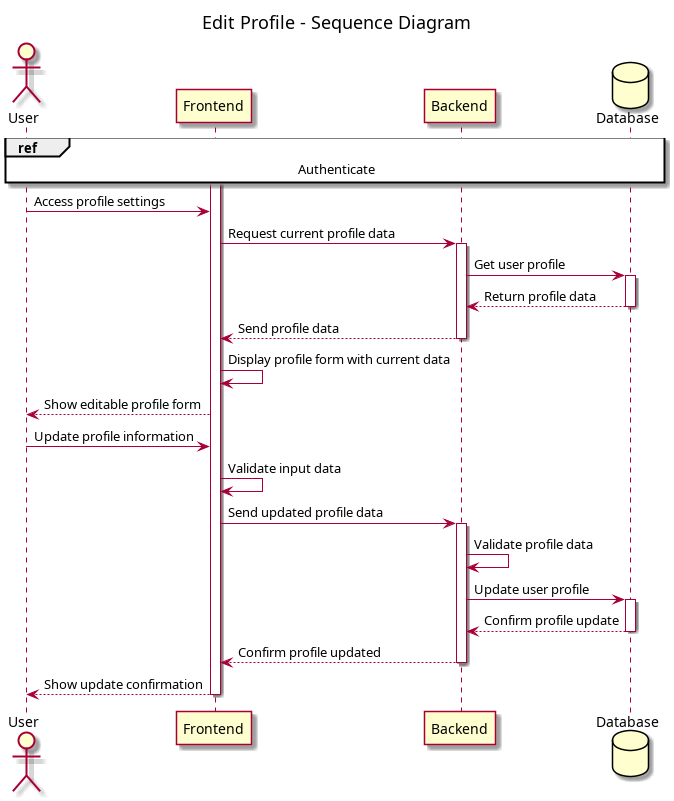
\includegraphics[width=0.9\textwidth]{conception/SprintV/sequence_diagrams/sequence_profileManagement_7_1_EditUserProfile.png}
\caption{Sequence Diagram: Edit User Profile}
\label{fig:seq_edit_profile}
\end{figure}

\begin{figure}[H]
\centering
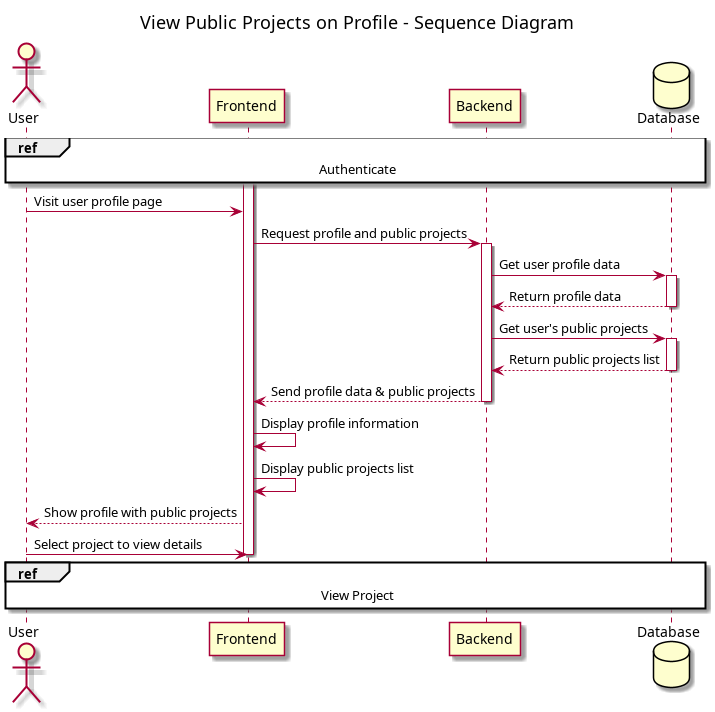
\includegraphics[width=0.9\textwidth]{conception/SprintV/sequence_diagrams/sequence_profileManagement_7_2_ViewPublicProjectsOnProfiles.png}
\caption{Sequence Diagram: View Public Projects on Profiles}
\label{fig:seq_view_public_projects}
\end{figure}

\section{Deliverables of Sprint V}

Sprint V delivered a comprehensive set of community interaction and profile management features, as demonstrated in the following implementation screenshots:

\begin{figure}[H]
\centering
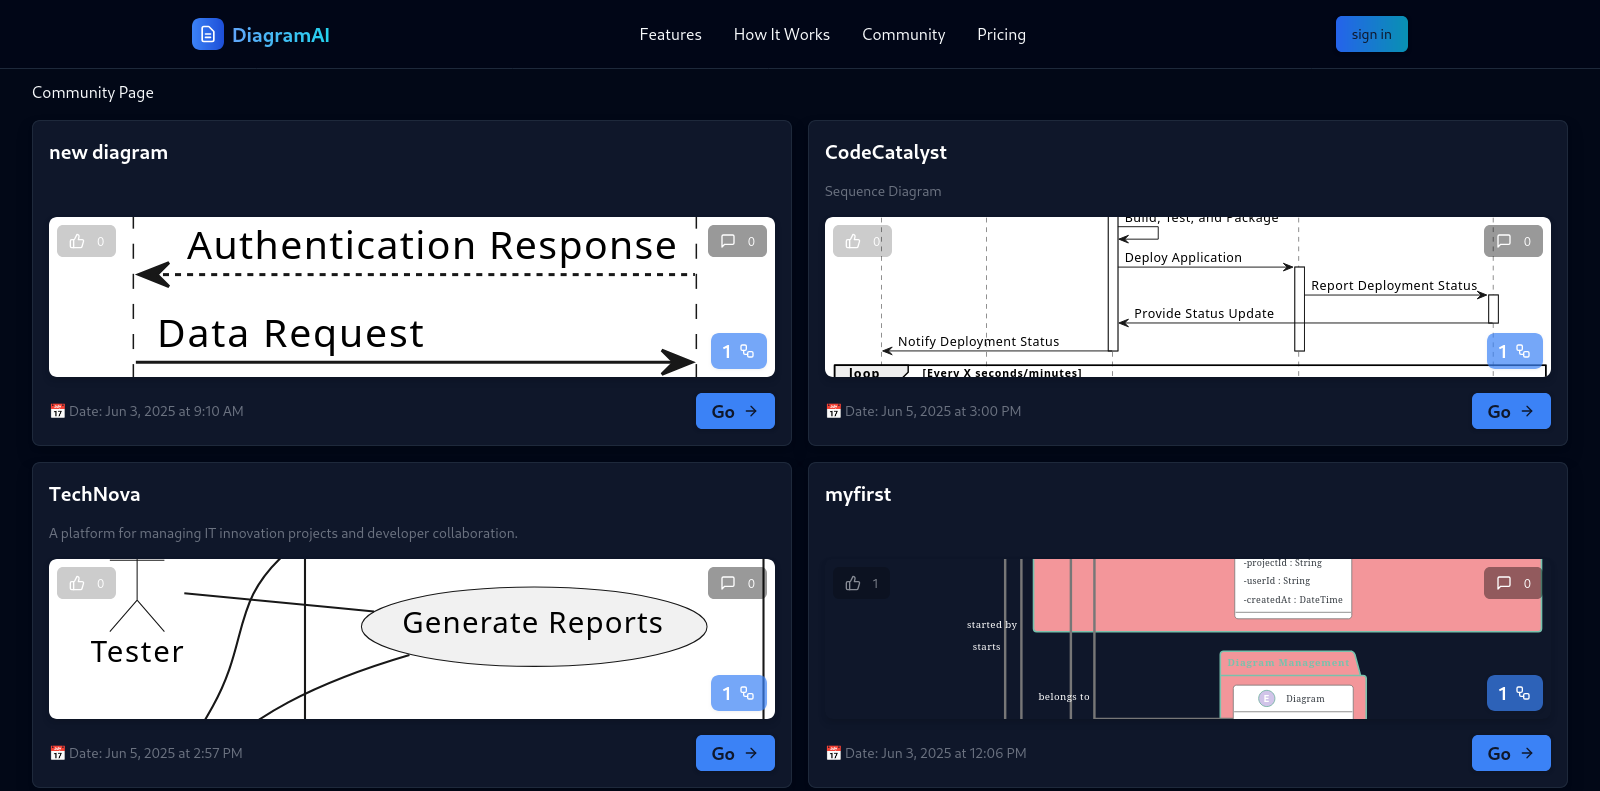
\includegraphics[width=0.9\textwidth]{screenshots/community1.png}
\caption{Community Exploration Interface - Main View}
\label{fig:community_main}
\end{figure}

The community exploration interface provides users with an intuitive way to discover and browse through available projects. The interface includes filtering options, search capabilities, and clear project previews with essential metadata.

\begin{figure}[H]
\centering
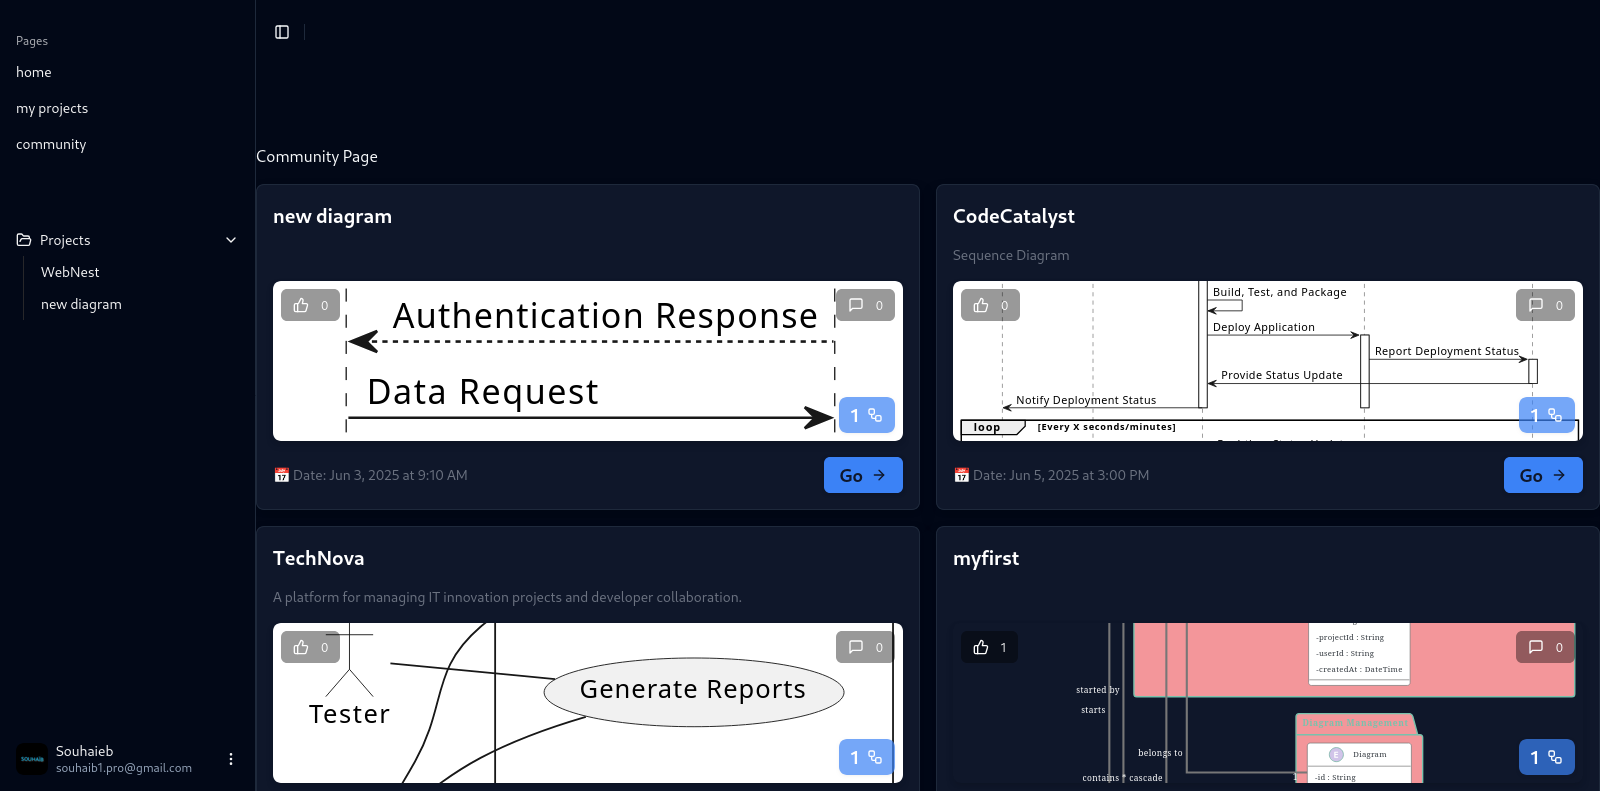
\includegraphics[width=0.9\textwidth]{screenshots/community2.png}
\caption{Community Exploration Interface - Project Details View}
\label{fig:community_details}
\end{figure}

The detailed project view within the community section showcases individual projects with comprehensive information, interaction buttons, and community engagement metrics.

\begin{figure}[H]
\centering
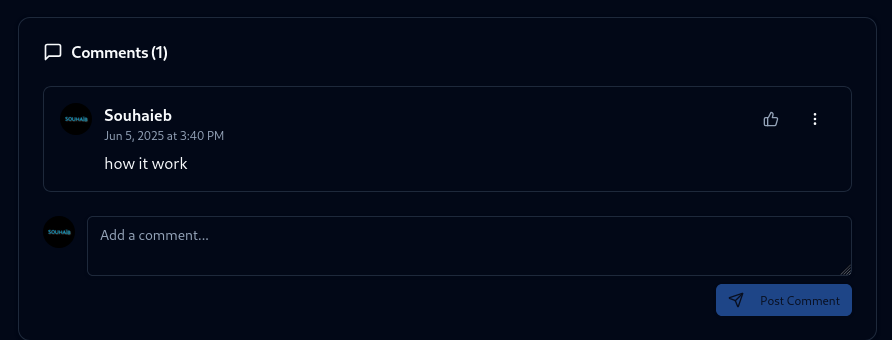
\includegraphics[width=0.9\textwidth]{screenshots/comment-section.png}
\caption{Comment Section Implementation}
\label{fig:comment_section}
\end{figure}

The comment section implementation demonstrates the full lifecycle of comment management, including creation, editing, deletion, and interaction features. Users can engage in meaningful discussions about projects through this comprehensive commenting system.

\begin{figure}[H]
\centering
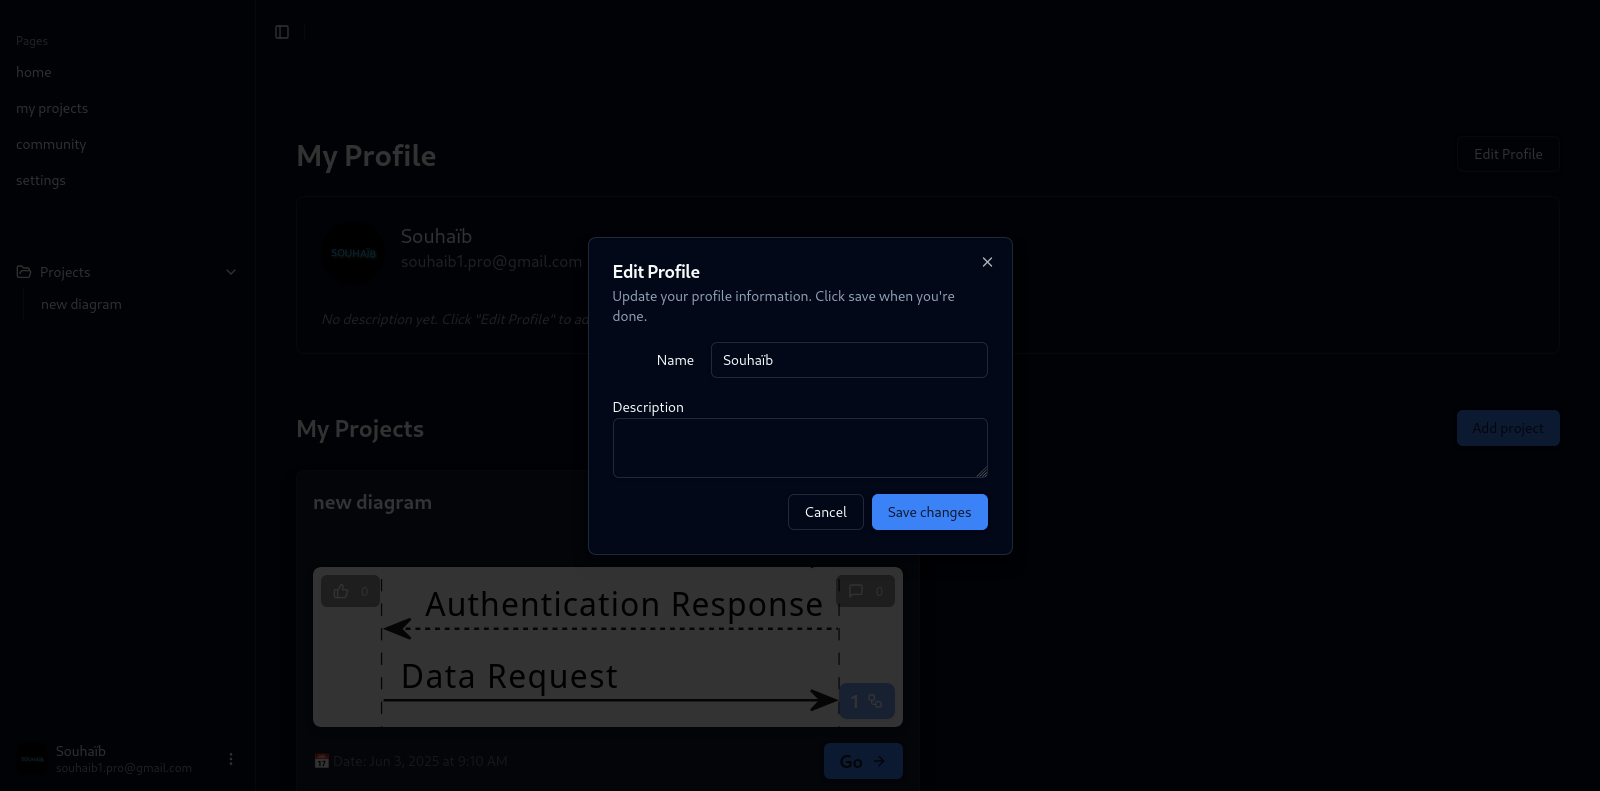
\includegraphics[width=0.9\textwidth]{screenshots/edit-profile.png}
\caption{Profile Editing Interface}
\label{fig:edit_profile}
\end{figure}

The profile editing interface allows users to maintain their account information, update personal details, and manage their public presence on the platform. The interface provides validation feedback and confirms successful updates.

\section{Retrospective of Sprint V}

The Sprint V retrospective revealed several key insights and areas for continuous improvement:

\textbf{What Went Well:}
\begin{itemize}
\item Successful implementation of comprehensive community interaction features
\item Effective collaboration between frontend and backend teams
\item Positive user feedback on comment management functionality
\item Smooth integration of profile management features
\item Strong adherence to planned timeline and deliverables
\end{itemize}

\textbf{Areas for Improvement:}
\begin{itemize}
\item Need for enhanced real-time notification system for community interactions
\item Optimization required for large-scale community project loading
\item User interface refinements based on usability testing feedback
\item Enhanced mobile responsiveness for community features
\end{itemize}

\textbf{Action Items for Future Sprints:}
\begin{itemize}
\item Implement real-time notifications for community engagement
\item Optimize database queries for improved performance
\item Conduct comprehensive usability testing sessions
\item Enhance mobile user experience across all features
\end{itemize}

\section{Conclusion}

Sprint V successfully transformed our platform into a collaborative community-driven ecosystem by implementing comprehensive interaction features and robust profile management capabilities. The delivery of community exploration, project commenting, liking mechanisms, and profile editing functionality establishes a solid foundation for user engagement and knowledge sharing.

The implementation demonstrates our commitment to building not just a diagramming tool, but a collaborative platform where users can learn from each other, share knowledge, and build upon collective expertise. The positive user feedback and successful integration of all planned features validate our approach and set the stage for continued platform evolution in subsequent sprints.